%!TEX root = ../../../../memoria.tex
\subsection{\paymentsCOM}\label{chapter:solucionimplementada:section:payment}
	
	Como se mencionó en la sección \ref{cap:solucionImplementada:section:dashboard:subsection:payment} \nameref{cap:solucionImplementada:section:dashboard:subsection:payment}, es relevante considerar varios métodos de pagos, sin embargo en el contexto de esta memoria solo se ha integrado a \PPPaymentProNAME


	\subsubsection{\PPPaymentProNAME}
		Anteriormente se habia indicado que este método permite mantener a los clientes dentro del \websiteINT durante el proceso completo de \paymentsCOM y \checkoutCOM. Básicamente se a implementado la aceptación de pago de tarjetas de crédito a través de un formlurio dentro del \websiteINT. La información necesaria para la transacción se ve en \refCodigo{source:javascript:checkout:payment:paypal_accept_payments}

		% JSON con la información necesaria para aceptar el pago con tarjetas de crédito
		%!TEX root = ../../../../memoria.tex

\medskip
\begin{lstlisting}[caption= Estructura de un \itemcollection, label=source:javascript:checkout:payment:paypal_accept_payments]
{	
	"intent": "sale",
	"payer":{
		"payment_method": "credit_card",
		"funding_instruments": [
			{
				"credit_card": {
					"number": "5500005555555559",
					"type": "mastercard",
					"expire_month": 12,
					"expire_year": 2018,
					"cvv2": 111,
					"first_name": "Betsy",
					"last_name": "Buyer"
				}
			}
		]
	},
	"transactions": [
		{
			"amount": {
				"total": "7.47",
				"currency": "USD"
			},
			"description": "This is the payment transaction description."
		}
	]
}
\end{lstlisting}

		De acá se desprende la información de la tarjeta

		\begin{itemize}
			\item Número.
			\item Tipo de Tarjeta.
			\item Mes en que expira la tarjeta.
			\item Año en que expira la tarjeta.
			\item \cvvTWOCOM.
			\item Nombre.
			\item Apellido.
		\end{itemize} 

		Toda esta información debe ser entregada por el cliente, con el fin de gestionar el pago. Sin embargo, se sabe que el tipo de tajeta puede ser determinado a partir de los 6 primeros dígitos del número de tarjeta \cite{online_investopedia_meaning_IIN}. 

		Los campos de expiración de tarjeta de crédito pueden ser confusos para decifrar si no son excritos exactamente como estan en las tarjetas de crédito. Algunos \websitesINT usan nombres de meses, mientras otros usan una combinación de \textit{nombre-número}, mientras otros usan solo números. La manera correcta de dar los campos de formato es simplemente poner los campos de la misma manera en que aparecen en la tarjeta de crédito (solamente números). Esto minimiza la confusión y mala interpretación por que el usuarios puede fácilmente verificar  los campos contra los de la tarjeta de crédito \cite{online_official_smashingmagazine_fundamental_guidelines_checkout_design}.

		Finalmente, se desarrolla el formulario de la \refFigura{figure:checkout:payment:paypal_payflow:form}, para que el cliente pueda efectuar el pago del producto y/o servicio.

		\begin{figure}[H]
			\centering
			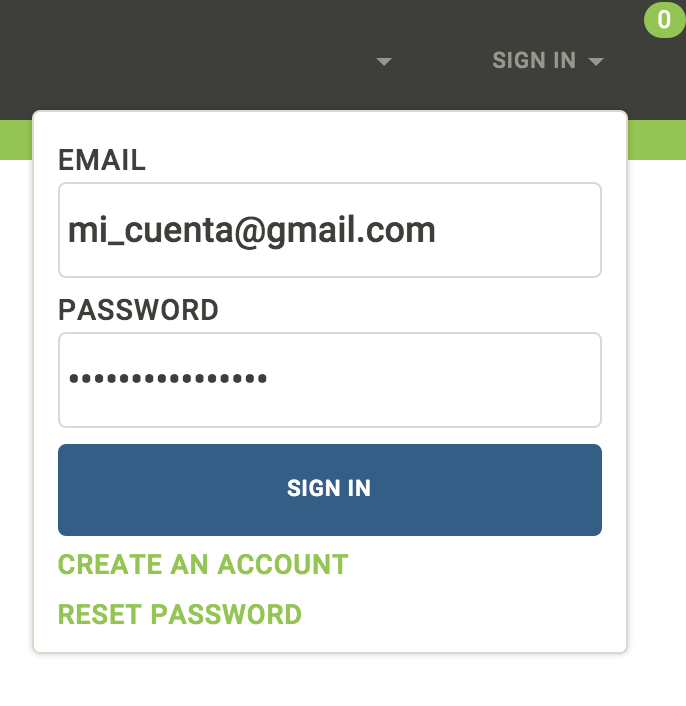
\includegraphics[width=0.6\textwidth]{figuras/checkout/payment/paypal_payflow/form.png}
			\caption{Formulario de la tarjeta de crédito para realizar el pago utilizando \PPPaymentProNAME.}
			\label{figure:checkout:payment:paypal_payflow:form}
		\end{figure}

		%TODO: agregar referencia a la interfaz de orde de compra.
		Una vez finalizado este proceso, se creara una orden de compra la cual podra ser consultado en la interfaz de ordenes.